% Sections/2_background_literature_review.tex
\section{Literature Review: UAV-Litter Solutions}

% For municipal technologies to be democratized, scalable, and adaptable to novel hazards, they must be grounded in open, reproducible research.

A literature review was conducted to understand how UAV-assisted systems currently address litter detection and cleanup. The review was framed around the specific context of this dissertation: disposable vape litter as hazardous micro-WEEE in pedestrianised UK urban spaces such as parks, towpaths and public squares.

UAV-assisted litter monitoring is often reported through object-detection results, but the practical workflow is broader than model inference. A useful system must acquire imagery, construct or access labelled data, train and evaluate a detector, locate detections in space, and communicate the result to the people responsible for cleanup. Figure~\ref{fig:uav_litter_pipeline} summarises this end-to-end UAV-litter pipeline.

\begin{figure}[H]
    \centering
    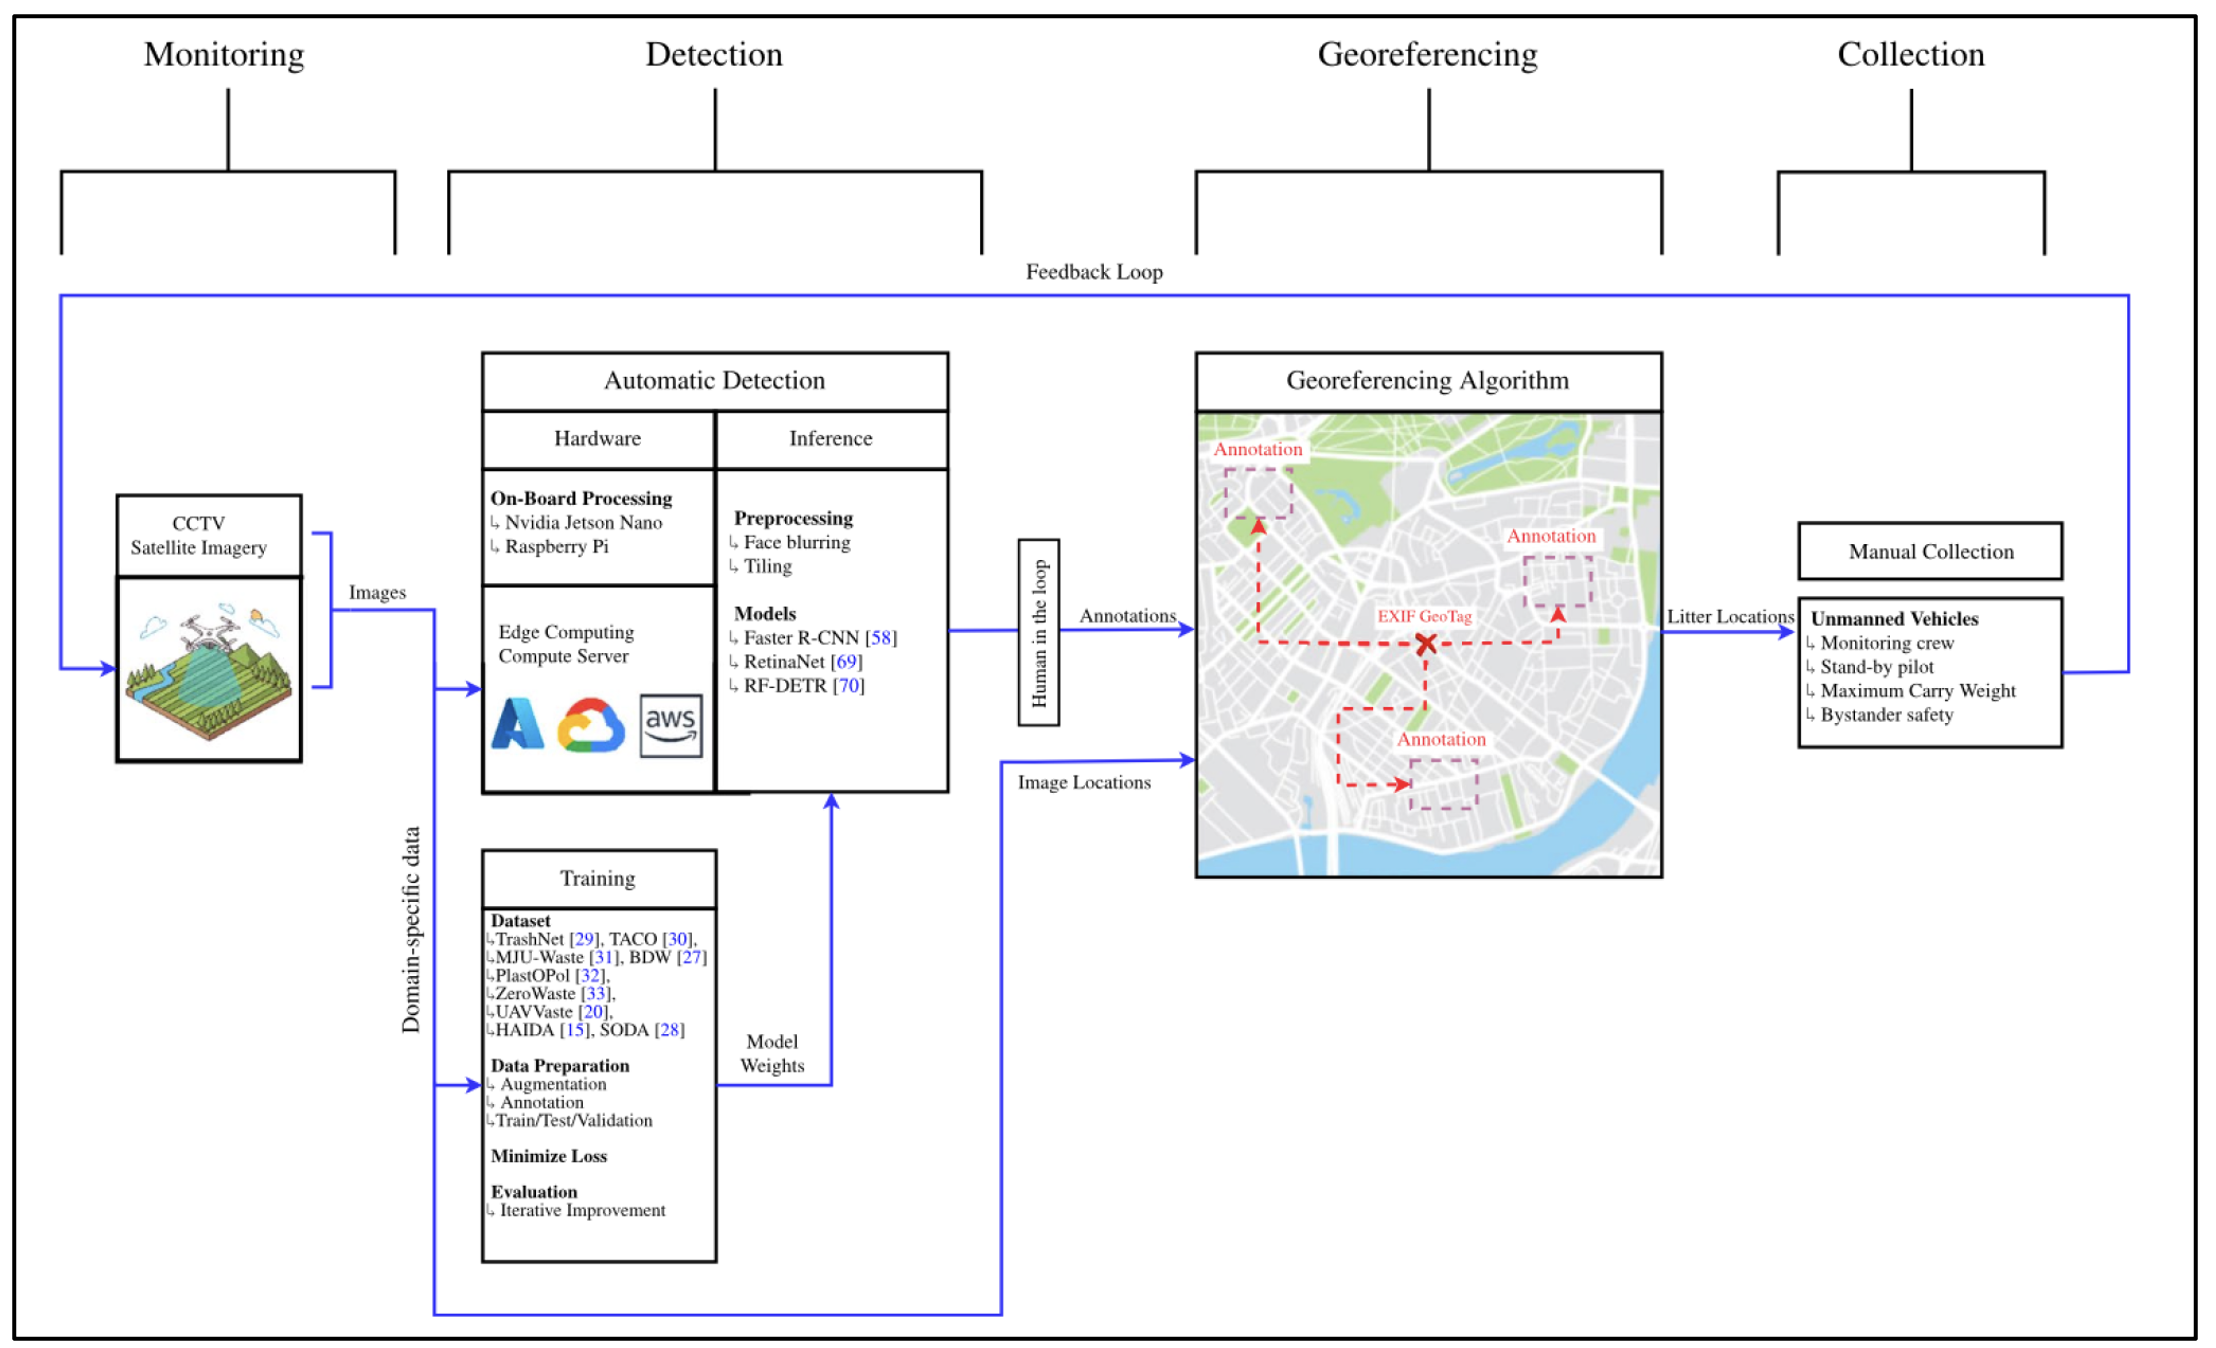
\includegraphics[width=0.8\linewidth]{Figures/UAV_Litter_Pipeline.png}
    \caption{UAV-litter pipeline from image acquisition to cleanup response.}
    \label{fig:uav_litter_pipeline}
\end{figure}

The review follows this pipeline: first datasets and annotation methods, then detector models and evaluation metrics, and finally post-detection localisation or cleanup support.

\subsubsection{Dataset}

The performance of an object detector is constrained by the dataset used to train and evaluate it. This matters especially for disposable vapes because they are small, visually diverse and easily confused with other elongated objects. A detector trained on generic litter classes may learn to identify bottles, cans or packaging, but that does not mean it can isolate vape litter as hazardous micro-WEEE.

Table~\ref{tab:datasets} compares the main datasets reviewed for this project. The review includes both non-UAV litter datasets and UAV-specific litter datasets because both groups are relevant. Non-UAV datasets show how litter has been labelled in computer vision more broadly, while UAV datasets show the visual constraints introduced by altitude, camera angle and small object scale. Dataset details were taken from the primary dataset sources \cite{trashnet_github,proenca2020taco,wang2020mjuwaste,cordova2022litter,bashkirova2021zerowaste,wang2018bottle,kraft2021uavvaste,liao2023automatic,pisani2024soda}.

\begin{table}[H]
\centering
\scriptsize
\begin{tabularx}{\textwidth}{p{0.15\textwidth}p{0.14\textwidth}p{0.14\textwidth}Xp{0.16\textwidth}p{0.16\textwidth}}
\toprule
\textbf{Dataset} & \textbf{Size} & \textbf{Viewpoint} & \textbf{Target classes / task} & \textbf{Annotation type / format} & \textbf{Annotation method} \\
\midrule
TrashNet (2017) & 2,527 images & Controlled non-UAV & Glass, paper, cardboard, plastic, metal, trash / classification & Image-level class labels; folders & Manual image sorting; no localisation. \\
\addlinespace
TACO (2020) & 1,500 images; 4,784 annotations & Ground-level in-the-wild & 60 litter categories / detection and segmentation & Polygon masks; COCO-style JSON & Manual polygon outlining of litter instances. \\
\addlinespace
MJU-Waste (2021) & 2,475 RGB-D images & Controlled non-UAV & General waste objects / segmentation & Pixel / polygon masks; VOC / COCO & Manual waste-object segmentation. \\
\addlinespace
PlastOPol (2021) & 2,418 images; 5,300 instances & Outdoor non-UAV & Single litter class / detection & Bounding boxes; detection labels & Manual boxing of litter instances. \\
\addlinespace
ZeroWaste (2021) & 4,503 images & Industrial conveyor & Industrial waste categories / detection and segmentation & Masks and boxes; dataset-specific & Object-level conveyor-waste annotation. \\
\addlinespace
UAV-BD / BDW (2021) & 25,407 images; 34,791 instances & UAV & Bottles / detection & Oriented bounding boxes; dataset-specific & Rotated bottle instances labelled with OBBs. \\
\addlinespace
UAVVaste (2021) & 772 images; 3,718 annotations & UAV & Generic rubbish / detection and segmentation & COCO boxes and polygons; COCO-like JSON & Hand-labelled UAV rubbish boxes and masks. \\
\addlinespace
HAIDA (2023) & 1,319 images; 6,475 instances & UAV / aerial & Marine debris / detection and monitoring & Object-level labels; format to verify & Aerial debris instances annotated; method to verify. \\
\addlinespace
SODA (2024) & 829 images; 6,719 annotations & UAV & Small litter objects / small-object detection & Bounding polygons; polygon labels & Tight polygon annotation for small UAV litter. \\
\bottomrule
\end{tabularx}
\caption{Litter dataset characteristics from literature, including annotation type and annotation method.}
\label{tab:datasets}
\end{table}

The literature shows that existing datasets are highly fragmented, differing in viewpoint, class taxonomy, annotation type and resolution, which prevents them from being used in synergy. Non-UAV datasets such as TrashNet, TACO, MJU-Waste, PlastOPol and ZeroWaste provide useful evidence for waste recognition, but their viewpoints and task definitions do not match UAV-oriented ground imagery. UAV-specific datasets such as UAVVaste, HAIDA and SODA are more relevant to aerial monitoring, but they focus on generic rubbish, bottles, marine debris or mixed small litter. No reviewed dataset isolates disposable vapes as a hazardous WEEE litter class, creating a distinct gap for a dedicated UAV-oriented vape dataset \cite{bartolo2026litterreview}.

\vspace{0.5em}
\noindent\textbf{Insight:} Existing UAV-litter datasets show that aerial litter detection is feasible, but they do not provide a vape-specific, metadata-rich dataset for hazardous micro-WEEE in UK urban environments.

The review also found limited evidence of environmental metadata in UAV-litter datasets. Standard labels describe class and location, but they rarely record surface, lighting, clutter, occlusion, viewpoint, motion blur or scale. This makes failure analysis difficult: if a detector fails on shadowed pavement or in grass, the dataset must store those conditions for the failure to be diagnosed. 

Annotation is also a major bottleneck. The reviewed datasets rely heavily on manual sorting, boxing or polygon tracing. Manual annotation is expected in many computer-vision datasets, but it becomes a stronger constraint for small, slender and visually ambiguous objects native to UAV-tasks. Disposable vapes often need tight outlines or accurate boxes because loose labels include large amounts of grass, pavement, leaves or gravel. This increases the risk that the detector learns background texture as part of the object.

\vspace{0.5em}
\noindent\textbf{Insight:} Current UAV-litter annotation practice remains largely manual, with limited literature supplementing datasets with environmental metadata.

\subsubsection{Deep-Learning Model Evaluation and Edge Constraints}

The model layer of UAV-litter research is dominated by one-stage object detectors, particularly You Only Look Once (YOLO) family models. This is appropriate for UAV and near-edge applications that require a balance between detection accuracy, inference speed, model size and power use \cite{kraft2021uavvaste,bartolo2026litterreview,ultralytics_detect_docs}.

\begin{table}[H]
\centering
\scriptsize
\begin{tabularx}{\textwidth}{p{0.12\textwidth}p{0.27\textwidth}p{0.20\textwidth}X}
\toprule
\textbf{Dataset} & \textbf{Models tested / discussed} & \textbf{Metric(s)} & \textbf{Best reported result / benchmark} \\
\midrule
TrashNet & Classification models; later YOLO-style detectors including YOLOv5. & Accuracy; detection mAP. & YOLOv5 derivative detection work reported mAP $\approx$ 0.95. \\
\addlinespace
TACO & Faster R-CNN, Mask R-CNN, YOLOv5 variants. & AP, AP50, recall, F1. & YOLOv5x reached AP 48.4 and AP50 63.3. \\
\addlinespace
MJU-Waste & Segmentation and RGB-D models. & Segmentation metrics. & Mainly useful as a segmentation/depth benchmark; 2,475 images and 2,525 instances. \\
\addlinespace
PlastOPol & Faster R-CNN, Mask R-CNN, YOLOv5x, YOLOv5s. & AP, AP50, AR, F1. & YOLOv5x reached AP 71.1 / AP50 84.9; YOLOv5s reached AP 62.4 / AP50 79.9. \\
\addlinespace
ZeroWaste & Mask R-CNN and detection/segmentation models. & AP, AP50, AP75. & Mask R-CNN reached AP 22.8, AP50 34.9 and AP75 24.4. \\
\addlinespace
UAV-BD / BDW & Faster R-CNN, YOLOv2, SSD, RRPN. & Accuracy, AP@0.5. & Faster R-CNN reached about 90\% accuracy; RRPN reached AP@0.5 $\approx$ 0.886. \\
\addlinespace
UAVVaste & YOLOv3, YOLOv4, YOLOv4-CSP, YOLOv4-tiny, EfficientDet, MobileNetV2 SSD. & mAP@50, mAP@50:95, AP/recall by size, FPS. & YOLOv4 FP32 reached mAP@50 = 0.785 and mAP@50:95 = 0.476; FP16 was similar at mAP@50 = 0.784. \\
\addlinespace
HAIDA & YOLOv4-Tiny-3l. & AP@0.5, inference performance. & AP@0.5 exceeded 70\%. \\
\addlinespace
SODA & YOLOv5, YOLOv8, Faster R-CNN. & mAP@0.5, AP by class/altitude. & YOLOv8 reached 89.4\% at 5m and 71.3\% at 30m with all-altitude training. \\
\bottomrule
\end{tabularx}
\caption{Model evaluation benchmarks across litter and UAV litter datasets.}
\label{tab:model_benchmarks}
\end{table}

Across the reviewed studies, direct comparison is difficult because dataset sizes, annotation types, target classes and evaluation splits vary. However, a clear pattern emerges: YOLOv3, YOLOv4, YOLOv5 and YOLOv8 appear more frequently than heavier two-stage or transformer-based detectors. Two-stage detectors such as Faster R-CNN remain useful benchmarks, and transformer-based detectors such as DETR provide an important alternative model family, but their higher compute requirements make them less common in UAV-litter work where real-time or near-real-time inference is a practical concern \cite{carion2020detr,zhu2021deformable_detr,kraft2021uavvaste,bartolo2026litterreview}.

\begin{table}[H]
\centering
\scriptsize
\begin{tabularx}{\textwidth}{p{0.18\textwidth} X p{0.34\textwidth}}
\toprule
\textbf{Model family} & \textbf{Use in litter / UAV-litter literature} & \textbf{Key characteristics} \\
\midrule
YOLOv3 / YOLOv4 & Common in earlier UAV-litter studies, including UAVVaste-style edge evaluations. & One-stage CNN detectors; real-time oriented; mature but older architectures. \\
\addlinespace
YOLOv5 & Widely used in applied litter and waste-detection studies. & Lightweight variants; strong open-source ecosystem; common practical baseline. \\
\addlinespace
YOLOv8 & Used in newer litter and small-object studies, including more recent UAV-litter comparisons. & Modern Ultralytics YOLO family; detection and segmentation support; useful recent baseline. \\
\addlinespace
YOLO11 & Newer Ultralytics detector, with limited representation in the reviewed UAV-litter literature. & Updated YOLO-family architecture; nano, small and medium scales support efficiency comparisons. \\
\addlinespace
YOLO26 & Current Ultralytics detector, not represented in the reviewed UAV-litter literature. & NMS-free inference, lighter detection head and updated small-target-aware training design. \\
\addlinespace
\bottomrule
\end{tabularx}
\caption{Detector families relevant to litter and UAV-litter detection.}
\label{tab:detector_families_lit}
\end{table}

Existing UAV-litter studies demonstrate that YOLO-style detectors are appropriate for aerial litter detection, but Table~\ref{tab:detector_families_lit} shows limited evidence of newer YOLO models being tested in this domain \cite{ultralytics_yolo11_docs,ultralytics_platform_docs}. Systematic comparisons between YOLO generations, model scales and input resolutions also remain underexplored. This matters because small-object UAV performance depends on whether a model can preserve enough visual detail while remaining computationally feasible, and different YOLO generations may behave differently on the same dataset.

\subsection{Metric Choice for UAV-Oriented Vape Detection}

Metric choice dictates how UAV-litter results are evaluated and compared, but the reviewed studies are not always consistent in reporting the full set of metrics. UAV literature often relies on AP and mAP because they evaluate performance across the precision-recall curve rather than at a single confidence threshold \cite{lin2014coco,ultralytics_metrics_docs}.

AP50 (Average Precision at a 0.5 Intersection-over-Union threshold) is widely reported in the reviewed studies, serving as a useful baseline for cross-literature comparison. In contrast, AP50--95 averages performance across multiple, stricter localisation thresholds and is less forgiving of loose bounding boxes. For small UAV litter, this distinction matters because a small spatial offset can strongly affect strict localisation metrics. Reporting both AP50 and AP50--95 therefore gives a clearer view of detector performance than relying on one score alone, especially where the operational goal is to locate an object for human retrieval.

\vspace{0.5em}
\noindent\textbf{Insight:} UAV-litter studies commonly use YOLO-family detectors and AP50-style metrics, making AP50 the most comparable benchmark across the literature. However, AP50 alone can overstate performance for small objects if localisation is loose. A vape-specific detector should therefore report AP50 for literature comparability, AP50--95 for stricter localisation and model selection, and precision/recall for operational interpretation.

\subsubsection{Localisation \& Cleanup Tasking}
The final gap is operational. UAV-litter studies often stop after detection metrics, georeferenced points or density maps. For example, UAVVaste and HAIDA demonstrate how UAV litter detection can be linked to coordinates, GIS layers or monitoring outputs using camera geometry, GPS and drone telemetry. These outputs are useful, but they do not fully explain how a cleaner or supervisor should act on the information. A map point alone does not show the evidence crop, confidence, hazard identity, task status or safe disposal route.

Mapping tools in other domains show that location-aware litter reporting is technically feasible. Citizen-science platforms such as Marine Debris Tracker demonstrate the value of app-based litter reporting with geotagged observations, but their focus is primarily marine based. OpenDroneMap provides open-source photogrammetry and mapping tools that can support UAV georeferencing, but is not litter-specific. OpenLitterMap shows how public litter observations can be mapped at scale, but litter points are generally treated as reporting records rather than cleanup tasks and do not distinguish vapes as a separate hazard \cite{marine_debris_tracker,opendronemap_docs,openlittermap}. This distinction matters: a vape is not operationally equivalent to a plastic wrapper because it requires separate WEEE handling and creates battery-fire risk if mixed with general waste.

\subsubsection{Literature Insights}
The literature reveals a critical baseline gap: the absence of a tailored, aerial-view dataset that isolates disposable vapes as a distinct micro-WEEE category in UK urban environments, alongside a need for systematic ablation studies on modern YOLO architectures. Beyond these immediate computational needs, the literature exhibits two deeper structural flaws. First, existing datasets suffer from fragmentation, manual annotation bottlenecks, and a lack of environmental metadata, making structured failure-mode analysis difficult. Second, current UAV-litter research often stops at raw spatial mapping and treats litter homogeneously, failing to provide the last-mile workflow integration required to manage vapes as hazardous e-waste.

While these insights expose \textit{what} is missing from the literature, they fail to uncover \textit{why} these deficits persist in practice. This fundamental gap prompted the core research question of this project:

\vspace{0.5em}
\noindent\textbf{How might we overcome the structural barriers to identifying and operationalizing disposable vapes as hazardous micro-e-waste in UAV-oriented imagery for UK urban environments?}

To address this, two practical investigations were required: an audit of current manual annotation tools to diagnose dataset creation bottlenecks, and an analysis of municipal cleaner workflows to determine how raw UAV detections can be practically translated into actionable cleanup interventions.
